\NextFile{OtherModules.html}
\chapter{MATSim input data (``MATSim containers'')}

Sorted alphabetically.

%%%%%%%%%%%%%%%%%%%%%%%%%%%%%%%%%%%%%%%%%%%%
%%%%%%%%%%%%%%%%%%%%%%%%%%%%%%%%%%%%%%%%%%%%
\section{"counts". Status: works for vsp and ivt}

\subsubsection{\textbf{Maintenance and Questions:}}

A. Horni, IVT (horni\_at\_IVT.baug.ethz.ch)

\subsubsection{\textbf{\textbf{Javadoc:
\\}}}

\href{http://www.matsim.org/javadoc/org/matsim/counts/package-summary.html}{www.matsim.org/javadoc/org/matsim/counts/package-summary.html}


\subsubsection{\textbf{\textbf{Config Parameters{}}}}

\href{http://www.matsim.org/javadoc/org/matsim/counts/package-summary.html#counts_parameters}{www.matsim.org/javadoc/org/matsim/counts/package-summary.html\#counts\_parameters}

\subsubsection{\textbf{In Brief:}}

MATSim can compare the simulated traffic volumes to traffic counts from the real world. Counts is the module that allows to
\begin{itemize}
	\item read some external file with traffic flow counts
	\item compare them automatically to the counts generated inside the matsim simulation
	\item submit the result to a kmz file which can be displayed inside google earth
\end{itemize}

There is a feature to re-scale the counts before comparison (for example if you are running the simulations with a 10\% sample).

\subsubsection{Comparison Data}

Prepare a file containing the real-world traffic counts. The file, e.g. named counts.xml, must follow the xml-format defined in \href{http://matsim.org/files/dtd/counts_v1.xsd}{counts\_v1.xsd}. An example of such a file can be found in MATSim at \href{http://matsim.svn.sourceforge.net/viewvc/matsim/matsim/trunk/examples/equil/counts100.xml?content-type=text%2Fplain}{examples/equil/counts100.xml}.

The file contains the following information:
\begin{itemize}
	\item For each link in the network for which traffic count information  is available, a count-element must exist. The count-element specifies  the link it refers to in its attribute 
\texttt{loc\_id}. In addition, an optional 
\texttt{cs\_id}  can be stored that may, for example, refer to the original id of the  counting station (for tracking back the origin of the data).
	\item In each count-element, 1 to 24 volume-elements can appear. Each volume-element contains the measured traffic count (attribute "
\texttt{val}") for an hour of the day (attribute "
\texttt{h}",  numbered from 1 to 24; 1 = 00:00-00:59, 2 = 01:00-01:59, etc). It is  not necessary that traffic counts are available for all 24 hours of a  day.
\end{itemize}


\subsubsection{Enabling Comparison in Configuration File}

Add the following lines to your configuration file:
\begin{verbatim}
<module name="counts">
  <param name="inputCountsFile" value="/path/to/counts.xml" />
  <param name="outputformat" value="txt,html,kml" />
</module>

\end{verbatim}

The comparison is automatically generated every 10th iteration.  Generated output is located in the output-directory of the iteration  (usually something like
\texttt{output/ITERS/it.10/}).


\subsubsection{Configuring the Counts Comparison}

The counts-module offers the following config-parameters:
\begin{itemize}
	\item 
\texttt{<param name="outputformat" value="txt,html,kml" />}
\\     The output format specifies in which format the comparison results are written to disk. It can be any combination of 
\texttt{txt}, html and 
\texttt{kml}. Multiple formats can be specified separated by commas. 
\texttt{txt} writes simple text-tables containing the values to a file. It is most useful to create custom graphs, e.g. in Excel. 
\texttt{html} creates a directory containing several html files, allowing to browse the results interactively. 
\texttt{kml} creates a file to be displayed in Google Earth. This last option only works if the \href{http://www.matsim.org/node/405}{correct coordinate system is set}.
	\item 
\texttt{<param name="countsScaleFactor" value="1.0" />}
\\     If you only simulate a sample of your population, the simulated  traffic volumes are likely lower than the real-world traffic counts. In  order to allow useful comparison, one can specify a factor by which the  simulated traffic volumes are multiplied. For example, if you simulate a  25\% sample of your full population, specify a countsScaleFactor  of 4.
	\item 
\texttt{<param name="distanceFilterCenterNode" value="2386" />
\\     <param name="distanceFiler" value="30000.0" />}
\\     If the traffic counts cover a larger area than the area being  simulated, the traffic counts outside your area will result in a bad  comparison. Instead of removing the traffic counts from the counts.xml,  you can specify a filter to only include some traffic counts from the  file in the comparison. To activate the filter, specify the id of a node  that acts as the center of a circle. The circle has the radius  specified in "
\texttt{distanceFilter}", the unit being the same unit as the length of links (i.e. usually meters).
\end{itemize}



\vfill\eject
%%%%%%%%%%%%%%%%%%%%%%%%%%%%%%%%%%%%%%%%%%%%
%%%%%%%%%%%%%%%%%%%%%%%%%%%%%%%%%%%%%%%%%%%%
\section{"facilities". Status: "user" version work in progress}

\textbf{Maintainer:} Andreas Horni

One may, or may not, use a separate file that contains "facilities" – essentially some kind of land use information.

The prototype for this is fairly old. But the final design is  somewhat different, and has not been fully executed. So I (kn) do  not know if this can currently be used as a non-developer.

\vfill\eject
%%%%%%%%%%%%%%%%%%%%%%%%%%%%%%%%%%%%%%%%%%%%
%%%%%%%%%%%%%%%%%%%%%%%%%%%%%%%%%%%%%%%%%%%%
\section{"households". Status: probably ready but nowhere used}

\textbf{Maintainer:} Christoph Dobler

An option to read a households file into matsim.

I (kn) don't know the exact status.

\vfill\eject
%%%%%%%%%%%%%%%%%%%%%%%%%%%%%%%%%%%%%%%%%%%%
%%%%%%%%%%%%%%%%%%%%%%%%%%%%%%%%%%%%%%%%%%%%
\section{"network". Status: ok}

\vfill\eject
%%%%%%%%%%%%%%%%%%%%%%%%%%%%%%%%%%%%%%%%%%%%
%%%%%%%%%%%%%%%%%%%%%%%%%%%%%%%%%%%%%%%%%%%%
\section{"network" (time dependent). Status: works for vsp}

\textbf{Maintenance:} G. Lämmel, VSP

MATSim provides the opportunity to model time dependent aspects of  the network explicitly. For each link in the network basic parameters  (i.e. freespeed, number of lanes and flow capacity) can be varied over  the time. So it is possible to model accidents or the like. One  particular area for this technique is the modeling of evacuation  scenarios.
In the case of an evacuation simulation the network has time dependent  attributes. For instance, large-scale inundations or conflagrations do  not cover all the endangered area at once.
In MATSim this time varying aspects are modeled as network change  events. A network change event modifies parameters of links in the  network at predefined time steps. The network change events have to be  provided in a XML file to MATSim.

A sample network change event XML file could look like:

\begin{lstlisting}{language=XML}
<?xml version="1.0" encoding="UTF-8"?>
<networkChangeEvents xmlns="http://www.matsim.org/files/dtd"  xmlns:xsi="http://www.w3.org/2001/XMLSchema-instance"  xsi:schemaLocation="http://www.matsim.org/files/dtd  http://www.matsim.org/files/dtd/networkChangeEvents.xsd">}

  <networkChangeEvent startTime="03:06:00">
    <link refId="12487"/>
    <link refId="12489"/>
    <link refId="12491"/>
    <freespeed type="absolute" value="0.0"/>
  </networkChangeEvent>

</networkChangeEvents>
\end{lstlisting}

This change event would set the freespeed of the links 
\texttt{12487, 12489, 12491} to 0 m/s at 
\texttt{03:06}  am (all values have to be provided in SI units). These values are valid  until the next network change event (if there is any) changes the  freespeed of link 
\texttt{12487, 12489, 12491} again. In this example the freespeed would be set to an absolute value. It is also possible to take the old 
\texttt{freespeed} value and multiply it by a factor. For dividing the old 
\texttt{freespeed} value by 2, the corresponding line of the network change event XML file would look like:
\\   
\texttt{<freespeed type="scaleFactor" value="0.5"/>}
\\  Besides changing the 
\texttt{freespeed}, one could also change the number of 
\texttt{lane}s:
\\   
\texttt{<lane type="absolute" value="2.0"/>}
\\  Or the flow capacity:
\\   
\texttt{<flowCapacity type="absolute" value="0.0"/>}
\\
\\  To make use of the network change events one has to define it in the  MATSim config file. Therefore the following two lines have to be added  in the network section of the config file:
\\
\texttt{<param name="timeVariantNetwork" value="true" />
\\  <param name="inputChangeEventsFile" value="path\_to\_ change\_events\_file" />}
\\
\\  Now one has just to start the controller with this config file and the network change events will be applied automatically.

It  seems that the ``absolute'' version of this module was never tested (and  may not work) with freespeeds other than zero. kai, oct'10



\vfill\eject
%%%%%%%%%%%%%%%%%%%%%%%%%%%%%%%%%%%%%%%%%%%%
%%%%%%%%%%%%%%%%%%%%%%%%%%%%%%%%%%%%%%%%%%%%
\section{"vehicles". Status: probably reads the file correctly, but does nothing else}

\textbf{Maintainer:} Michael Zilske (within limits of DFG/MUC project; possibly pt project)

\vfill\eject
%%%%%%%%%%%%%%%%%%%%%%%%%%%%%%%%%%%%%%%%%%%%
%%%%%%%%%%%%%%%%%%%%%%%%%%%%%%%%%%%%%%%%%%%%

\chapter{Other configurable modules}

% I now think that there should be
% * matsim containers (population, network, facilities, households, ...)
% * mobsims
% * other
% kai, oct'13



Modules are loosely defined by their corresponding entry in the config file.

They are also sorted in the same sequence (which is done by the machine, not by content).

Note that individual config options are often explained inside the config section of the log file.

Config file modules that just define files/directories are, as a tendency, not explained here.Note that strategy modules (such as ReRoute, Planomat) are described in a separate section.

Maintainers are mentioned as far as possible, but they are \emph{not} responsible for answering arbitrary service requests.

\vfill\eject
%%%%%%%%%%%%%%%%%%%%%%%%%%%%%%%%%%%%%%%%%%%%
%%%%%%%%%%%%%%%%%%%%%%%%%%%%%%%%%%%%%%%%%%%%
\section{"global". Status: indispensable}

\textbf{"Maintainer":} Marcel Rieser

"Global" information. Arguably should be merged with "controler" section.

\vfill\eject
%%%%%%%%%%%%%%%%%%%%%%%%%%%%%%%%%%%%%%%%%%%%
%%%%%%%%%%%%%%%%%%%%%%%%%%%%%%%%%%%%%%%%%%%%
\section{"JDEQSim".  Status: works for ivt}

\textbf{Maintainer:} Rashid Waraich

\subsubsection{Overview}

JDEQSim (Java Deterministic Event Driven Queue Based Simulation) has the following properties and features:
\begin{itemize}
	\item it is based on a discrete event simulation model
	\item traffic simulation is based on a queue model for streets (FIFO: first in first out)
	\item deadlock prevention is achieved by squeezing vehicles
	\item gaps  generated at front of queue propagate backwards with a speed called  'gapTravelSpeed' resulting in a more realistic traffic model
\end{itemize}

\subsubsection{Usage}

Insert  a new module called 'JDEQSim' into the config XML file. All parameters  are optional and have default values (shown below), never the less it  could be helpful to know their meaning and physical units.
\begin{lstlisting}{language=XML}
<module name="JDEQSim">
    <param name="endTime" value="00:00:00"   />
    <param name="flowCapacityFactor" value="1.0"   />
    <param name="storageCapacityFactor" value="1.0"   />
    <param name="minimumInFlowCapacity" value="1800"   />
    <param name="carSize" value="7.5"   />
    <param name="gapTravelSpeed" value="15.0"   />
    <param name="squeezeTime" value="1800"   />
</module>
\end{lstlisting}

The mobsim type now  also needs to be defined in the controler section of the config  file. See comments in config dumps in logfiles.

The  'endTime' defines the time of the last event of the simulation. If it is  set to '00:00:00', no end time is defined and the simulation will stop,  when the last event of the simulation has been processed. The (scaling)  parameters  'flowCapacityFactor' and 'storageCapacityFactor' can  be used as with mobSim and have no unit. The 'minimumInFlowCapacity'  defines for all roads the minimum number of cars, which could enter the  road per hour, for the congestion less case. The 'carSize' parameter  allows to set the size of a car in meters. The 'gapTravelSpeed'  parameter defines the speed of gaps in [m/s]. Finally the 'squeezeTime'  is used for deadlock prevention and defines, how long a car should wait  at maximum for entering the next road before deadlock prevention is  turned on (unit: seconds).

The 'minimumInFlowCapacity' is a  parameter, which was not published in the C++ DEQSim, but only used  interally and was hardcoded to the value 1800 vehicles per hour. This  value was estimated from literature assuming that independently from the  speed limit of a road the minimum interval between two vehicles is 2  seconds (inverse of 1800 vehicles per hour). This factor does not need  to be changed, when the 'flowCapacityFactor' is changed, as the scaling  is automatically done internally. The reason for publishing this factor  is to make it possible for users to adapt this factor, if they want to  use a different minium inflow capacity based on their model estimations.

\subsubsection{Hints}
\begin{itemize}
	\item You might consider turning on the module  'parallelEventHandling' when using JDEQSim, as often JDEQSim can make  much better use of this module than QueueSim (as JDEQSim is faster).
	\item If you are getting lots of breakdowns, consider using smaller squeezeTime (e.g. 10 seconds or lower)
\end{itemize}

\subsubsection{Requirements for the Plans XML File}

\begin{itemize}
	\item For each person the 'end\_time' of the first act must be defined ('dur' is ignored).
	\item For the other acts of a person either 'dur' or 'end\_time' needs to be defined
	\item If both 'dur' and 'end\_time' are defined, then only the one which occurs earlier is considered
\end{itemize}

\subsubsection{Differences between MobSim and JDEQSim}
\begin{itemize}
	\item QueueSim  uses a simulation approach called 'fixed-increment time advance'  instead of 'next-event time advance', which makes it much slower than  JDEQSim for high resolution networks.
	%%\item JDEQSim allows  squeezing of vehicles to resolve possible deadlocks. Deadlock prevention  in QueueSim is (traditionally) dealt with by removing vehicles from the  network or squeezing.
%
% squeezing has been possible in the qsim for many years now. kai, oct'13
	\item JDEQSim models gap travel times more realistically than QueueSim, where this feature is missing.
\end{itemize}




\subsubsection{Further Reading}

This implementation is based on the micro-simulation described in the following paper:

Charypar, D., K. Nagel and K.W. Axhausen (2007) An event-driven queue-based microsimulation of traffic flow, \emph{Transportation Research Record}, \textbf{2003}, 35-40.Order \href{http://trb.metapress.com/content/j2118065485r4611/?p=4f63e25a261d48d99eeebea19b494e24&amp;pi=0}{here}.

Some  Java specific implementation aspects and performance tests of JDEQSim  and parallelEventHandling are described in the following paper:

Waraich,  R., D. Charypar, M. Balmer and K.W. Axhausen (2009) Performance  improvements for large scale traffic simulation in MATSim, paper  presented at the \emph{9$^th$ Swiss Transport Research Conference}, Ascona, September 2009. Download from \href{http://www.ivt.ethz.ch/vpl/publications/reports/ab565.pdf}{here}.

\vfill\eject
%%%%%%%%%%%%%%%%%%%%%%%%%%%%%%%%%%%%%%%%%%%%
%%%%%%%%%%%%%%%%%%%%%%%%%%%%%%%%%%%%%%%%%%%%
\section{"controler". Status: indispensable}

\subsubsection{\textbf{Maintenance and Questions}}

Marcel Rieser, Senozon AG (rieser\_at\_senozon.com)

\subsubsection{\textbf{Javadoc}}

\href{http://www.matsim.org/javadoc/org/matsim/core/controler/package-summary.html}{www.matsim.org/javadoc/org/matsim/core/controler/package-summary.html}



\subsubsection{Config Parameters}

\href{http://www.matsim.org/javadoc/org/matsim/core/controler/package-summary.html#controler_parameters}{www.matsim.org/javadoc/org/matsim/core/controler/package-summary.html\#controler\_parameters}


\subsubsection{\textbf{\textbf{In Brief}}}

Central module to run matsim. Specifies, for example, the number of iterations.



\subsubsection{Notes}

See \href{http://matsim.org/node/398}{here} for some instructions how to use an external executable as mobsim.

\vfill\eject
%%%%%%%%%%%%%%%%%%%%%%%%%%%%%%%%%%%%%%%%%%%%
%%%%%%%%%%%%%%%%%%%%%%%%%%%%%%%%%%%%%%%%%%%%
% I think this is now fully a contrib.  kai, oct'13
%%\section{"evacuation"(-ivt). Status: ??}

%%Evacuation code used by IVT; please note that IVT and VSP use different evacuation codes.

%%Maintained by C. Dobler.

%%I (kn) don't know how this works

%%\vfill\eject
%%%%%%%%%%%%%%%%%%%%%%%%%%%%%%%%%%%%%%%%%%%%
%%%%%%%%%%%%%%%%%%%%%%%%%%%%%%%%%%%%%%%%%%%%
% I think this is now fully a contrib.  kai, oct'13
%%\section{"evacuation"(-vsp). Status: works if you know what you are doing}

%%(Note that VSP and IVT use different evacuation packages.)

%%\subsubsection{\textbf{Maintenance and Questions}}

%%G. Lämmel, TU Berlin

%%\subsubsection{\textbf{Javadoc}}

%%\href{http://www.matsim.org/javadoc/org/matsim/evacuation/package-summary.html}{http://www.matsim.org/javadoc/org/matsim/evacuation/package-summary.html}


%%\subsubsection{\textbf{\textbf{Config Parameters{}}}}

%%\href{http://www.matsim.org/javadoc/org/matsim/evacuation/package-summary.html#evacuation_parameters}{http://www.matsim.org/javadoc/org/matsim/evacuation/package-summary.html\#evacuation\_parameters}

%%\subsubsection{\textbf{\textbf{In Brief}}}

%%I (kn) can't say how this works. There is, at this point, neither documentation nor funding.

%%\vfill\eject
%%%%%%%%%%%%%%%%%%%%%%%%%%%%%%%%%%%%%%%%%%%%
\section{"parallelEventHandling". Status: works for ivt and vsp}

\textbf{Maintainer:} Rashid Waraich

see details \href{http://matsim.org/node/238}{here}.



\vfill\eject
\section{"planCalcScore". Status: nearly indispensible}

\textbf{Maintainer:} Marcel Rieser

This module contains the definitions for the utility function.

Some help for it should be in the tutorials.

There is also some description in the "scoring function" section of the documentation.

\vfill\eject
\section{"qsim" (parallel version). Status: looks promising}

Responsible: C. Dobler, IVT

Analysis of performance and structure of (non parallel) QueueSim shows:
\begin{itemize}
	\item Simulation of movement on links and over nodes is most time consuming.
	\item Within a timestep actions on nodes and links can be simulated on parallel threads with low additional synchronization effort.
\end{itemize}

The  parallel QueueSim is based on the existing QueueSim and can be used by  just adding a new parameter to a scenario configuration file (see  below).

First performance measurements show promising results.

Working paper will be published in Q2 2010.

\begin{figure}[htp]
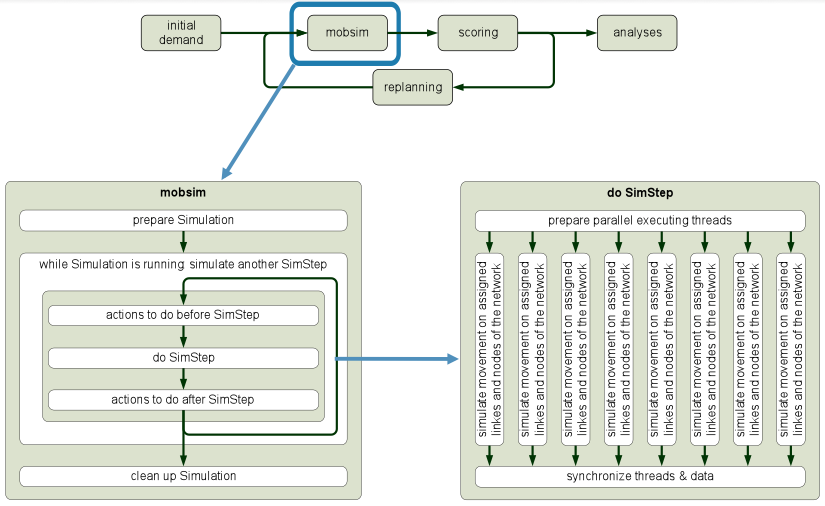
\includegraphics[width=\textwidth]{figures/qsimParallel/parallelqsim.png}
\caption{Design of the parallel qsim}
\end{figure}

The config option presumably is:
\begin{verbatim}
<module name="qsim">
   ...
   <param name="numberOfThreads" value="5"/>
</module>

\end{verbatim}

Any number of threads larger than $1$ triggers the use of the parallel version.

\vfill\eject
\section{"qsim". Status: works but is not very transparent}

\sout{If you do \textbf{\emph{not}} put a "qsim" section into the config file, the system will use the default "simulation" (look there).}

"qsim"  is what we use for new features such as public transit or  signalsystems. "New features" implies "unstable". Use only  if you have to.

Also see \href{http://www.matsim.org/javadoc/org/matsim/ptproject/qsim/package-summary.html}{www.matsim.org/javadoc/org/matsim/ptproject/qsim/package-summary.html}

\subsubsection{Some calibration hints, especially when the main mode is not "car"}

The (exit) flow capacity of a link is:
\begin{verbatim}
capacity_value_of_link / capacity_period_of network * flow_capacity_factor

\end{verbatim}

where
\begin{itemize}
	\item the capacity value of the link is given by the link entry in the network file
	\item the  capacity period of the network is given at the beginning of the "links"  section in the network file. Normally set to one hour
	\item the flow capacity factor is given in the qsim config group
\end{itemize}

The storage capacity of a link is:
\begin{verbatim}
(length_of_link * number_of_lanes_of_link / effective_cell_size) * storage_capacity_factor

\end{verbatim}

where
\begin{itemize}
	\item the length of the link is given by the link entry in the network file
	\item the number of lanes of the link is given by the link entry in the network file
	\item the effective cell size is given at the beginning of the "links" section in the network file. Normally set to 7.5m
	\item the storage capacity factor is given in the qsim config group
	\item There  is also an effective lane width, also at the beginning of the "links"  section in the network file, normally set to 3.75m. See below for  its use.
\end{itemize}

This is most useful if you have something else than  cars, for example pedestrians. Let us assume an effective lane  with of 0.4m and an effective cell size also of 0.4m. This would  lead to a maximum density of 0.4*0.4=0.16persons/$m^2$, not totally  unrealistic.

If, now, a link has an area of $200m^2$ and a length of 50m, then it would obtain
\begin{verbatim}
number_of_lanes = area / length / effective_lane_width = 200 / 50 / 0.4 = 10

\end{verbatim}

Note that, in the end, the lane width is not used by the  dynamics; all the meaning is subsumed in the number of lanes. The  storage capacity comes out as
\begin{verbatim}
storage_capacity = number_of_lanes * length / effective_cell_size

\end{verbatim}

in the above example
\begin{verbatim}
= 10 * 50 / 0.4 = 1250 .

\end{verbatim}

This is, naturally, the same as dividing the 200m\textasciicircum2 of the link by the 0.16persons/$m^2$.

The effective lane width might be used by the visualization (unclear if this is the case).

\vfill\eject
%%%%%%%%%%%%%%%%%%%%%%%%%%%%%%%%%%%%%%%%%%%%
%%%%%%%%%%%%%%%%%%%%%%%%%%%%%%%%%%%%%%%%%%%%%%
%%\section{"roadpricing".  Status: works for vsp}

%%\textbf{Maintainer:} Michael Zilske

%%The roadpricing module provides functionality to simulate different road-pricing scenarios in MATSim.

%%Documentation can be found at:
%%\begin{itemize}
%%	\item \href{http://ci.matsim.org:8080/job/MATSim_contrib_M2/org.matsim.contrib$roadpricing/javadoc/?}{http://ci.matsim.org:8080/job/MATSim\_contrib\_M2/org.matsim.contrib\$roadpricing/javadoc/?}
%%\end{itemize}

%%Publications using this module:
%%\begin{itemize}
%%	\item \href{https://svn.vsp.tu-berlin.de/repos/public-svn/publications/vspwp/2007/07-14/}{https://svn.vsp.tu-berlin.de/repos/public-svn/publications/vspwp/2007/07-14/}
%%	\item \href{https://svn.vsp.tu-berlin.de/repos/public-svn/publications/vspwp/2008/08-01/}{https://svn.vsp.tu-berlin.de/repos/public-svn/publications/vspwp/2008/08-01/}
%%	\item \href{https://svn.vsp.tu-berlin.de/repos/public-svn/publications/vspwp/2008/08-08/}{https://svn.vsp.tu-berlin.de/repos/public-svn/publications/vspwp/2008/08-08/}
%%	\item \href{https://svn.vsp.tu-berlin.de/repos/public-svn/publications/vspwp/2010/10-03/}{https://svn.vsp.tu-berlin.de/repos/public-svn/publications/vspwp/2010/10-03/}
%%\end{itemize}


%%\vfill\eject

% roadpricing is no longer core but now a contrib.  kai, oct'13

%%%%%%%%%%%%%%%%%%%%%%%%%%%%%%%%%%%%%%%%%%%%
%%%%%%%%%%%%%%%%%%%%%%%%%%%%%%%%%%%%%%%%%%%%
\section{"lanes". Status: works}

\textbf{Maintainer:} Dominik Grether

Make sure you read \url{http://svn.vsp.tu-berlin.de/repos/public-svn/publications/vspwp/2012/12-03/} before you use the lanes module to understand effects on the queue model.

\subsection{Configuration}

To use lanes make sure that the following parameters are set

\begin{verbatim}
<module name="controler" >	
	...
	<param name="enableLinkToLinkRouting" value="true" />
	<param name="mobsim" value="qsim" />
	...
</module>

<module name="qsim" >
	...
	<param name="numberOfThreads" value="1" />
	...
</module>

<module name="scenario" >
	...
	<param name="useLanes" value="true" />
	...
</module>

<module name="network" >
	...
	<param name="laneDefinitionsFile" value="PATH TO FILE" />
	...
</module>
\end{verbatim}

\subsection{Capacity interpretation of lanes}

In principle a lane is similar to the representation of a link in the queue model. 

The (exit) flow capacity of a lane is:

\begin{verbatim}
capacity_value_of_lane / flow_capacity_factor
\end{verbatim}

where
\begin{itemize}
	\item the capacity value of the lane is given in the laneDefinitions\_v2.0.xsd compatible input file
	\item the flow capacity factor is given in the qsim config group
\end{itemize}

The storage capacity of a lane is

\begin{verbatim}
(length_of_lane * no_of_represented_lanes / effective_cell_size) * storage_capacity_factor
\end{verbatim}

where
\begin{itemize}
	\item the length of the lane is calculated by the value of the \verb$<startsAt meterFromLinkEnd=10 />$ element within the \verb$<lane>$ element of the laneDefinitions\_v2.0.xsd file format. \\
		\begin{itemize}
			\item If the lane ends at the end of the link, its length is simply the \verb$meterFromLinkEnd$ value
			\item If the lane leads to other downstream lanes, its length is calculated from the distance between the position on the link the downstream lanes start from and the \verb$meterFromLinkEnd$ value of the lane. 
		\end{itemize}
	\item the number of represented lanes is the value of the \verb$number$ attribute of the  \verb$<representedLanes>$ element of the laneDefinitions\_v2.0.xsd file format.
	\item the storage capacity factor is given in the qsim config group
\end{itemize}


\vfill\eject
%%%%%%%%%%%%%%%%%%%%%%%%%%%%%%%%%%%%%%%%%%%%
%%%%%%%%%%%%%%%%%%%%%%%%%%%%%%%%%%%%%%%%%%%%
\section{"signalsystems". Status: works}

\textbf{Maintainer:} Dominik Grether

The signal systems module provides functionality to simulate traffic  lights with MATSim. It is recommended to use a nightly build that is  younger than 04-19-2011, i.e. revision 15081.

Have a look at the tutorial at \href{http://matsim.org/node/732}{http://matsim.org/node/732}.

The starting point of the technical documentation is
\begin{itemize}
	\item \href{http://www.matsim.org/javadoc/org/matsim/signalsystems/package-summary.html}{http://www.matsim.org/javadoc/org/matsim/signalsystems/package-summary.html}
\end{itemize}

Note that there are links to continuative documentation at the bottom of the package-summary.html www page.

MATSim ships with a tutorial that shows you how to set up a traffic  light scenario. The network and traffic light configuration of the  turorial is shown in the slides attached to this page. The network and  code can be found in the folder  tutorial/unsupported/example90TrafficLights in the nightly build. The  code examples are divided into several classes:
\begin{itemize}
	\item CreateSimpleTrafficSignalScenario.java: Uses traffic signals  without lanes and creates the traffic lights at nodes 3, 4, 7 and 8.
	\item CreateTrafficSignalScenarioWithLanes.java: Uses traffic signals with lanes and creates the traffic lights at nodes 2 and 5.
\end{itemize}



Publications using this module:
\begin{itemize}
	\item \href{https://svn.vsp.tu-berlin.de/repos/public-svn/publications/vspwp/2008/08-24/}{https://svn.vsp.tu-berlin.de/repos/public-svn/publications/vspwp/2008/08-24/}
	\item \href{https://svn.vsp.tu-berlin.de/repos/public-svn/publications/vspwp/2011/11-12/}{https://svn.vsp.tu-berlin.de/repos/public-svn/publications/vspwp/2011/11-12/}
	\item \href{https://svn.vsp.tu-berlin.de/repos/public-svn/publications/vspwp/2011/11-08/}{https://svn.vsp.tu-berlin.de/repos/public-svn/publications/vspwp/2011/11-08/}
\end{itemize}This documentation is missing an  explanation of the "lanes" option. Please ask if you need this  (separate "lanes" for separate turning movements).



%%%\includegraphics{User%27s%20Guide_files/application-pdf.png}\href{http://www.matsim.org/uploads/384/signals_tutorial_0.pdf}{signals\_tutorial.pdf} & 77.72 KB
%%\end{tabular}

\vfill\eject
\section{"simulation". Status: should work}

This  was essentially the production of the queue simulation until Nov/2010.  The "qsim" was then forked out for further development. Unfortunately,  this fork was done somewhat too late, so "simulation" is not exactly the  stable version that was used over many years, but something that is  already somewhat modified, and was not used very much after that.  (Please let us know if you have problems.)

Note that you will get a "simulation" section in the log file even if  you have selected a different mobsim (such as qsim or jdqsim).

There used to be an option to start an external mobsim. This still seems to be there but the syntax is a bit awkward:
\begin{verbatim}
<module name="controler" >
   ...
   <param name="mobsim" value="null" />
</module>
<module name="simulation" >
   <param name="externalExe" value="<path-to-executable>" />
</module>


\end{verbatim}

I.e. you need to specify that you are \emph{not} using the (queue)Simulation, but then set a parameter inside the (queue)Simulation config block.

\vfill\eject
\section{"strategy". Status: indispensable}

\textbf{Maintainer:} Marcel Rieser ("core")

See \href{http://matsim.org/node/478}{here}.

\vfill\eject
\section{"transit" (public transport).  Status: works}

A  public transport system is simulated and integrated on a fine scale  with both the traffic simulation and the behavior of the artificial  population.

Agents who use transit determine a route to their destination based  on the transit schedule. Transit vehicles are moved on the road network  in accordance with the traffic flow model, i.e. they may get stuck in  congestion and fail to keep their schedule. Agents getting on and off  transit vehicles cause realistic delays.

A transport mode decision model is implemented which allows agents to  switch their choice of driving a car or using transit based on the  relative utility of the two modes. The disutility of travel time, which  this model takes into account, is based on actual travel times taken  from the simulation.

See the \href{http://matsim.org/docs/tutorials/transit}{tutorial}. This requires quite some additional input.

\subsubsection{Reference}

M. Rieser, K. Nagel; \textbf{Combined agent-based simulation of private car traffic and transit}; IATBR 2009

\vfill\eject
\section{"travelTimeCalculator". Status: nearly indispensable}

\textbf{Maintainer:} Marcel Rieser ("core")

"router" and "travelTimeCalculator" are separate in matsim, so that  they can be configured separately. They refer to each other,  though.

\vfill\eject
%%%%%%%%%%%%%%%%%%%%%%%%%%%%%%%%%%%%%%%%%%%%
%%%%%%%%%%%%%%%%%%%%%%%%%%%%%%%%%%%%%%%%%%%%
\section{"vspExperimental". Status: used by VSP}

This  section defines switches that are used at VSP or when collaborating  with VSP. There are experimental and may we withdrawn without  notice.

\subsubsection{vsp defaults}

I (kn) am in the process of defining some defaults that everybody at VSP should be using. These can be switched on by:
\begin{verbatim}
<module name="vspExperimental" >
   <param name="vspDefaultsCheckingLevel" value="abort" />
   ...
</module>

\end{verbatim}

This will make the code abort when these defaults are violated.

The number of vsp defaults will grow over time. This may have  the effect that some config file that used to be working for you in the  past may not work any more after an svn update. I will try to  communicate such changes, but will sometimes fail to do so. In any  case, if you encounter an abort because of a vsp defaults violation,  please
\begin{itemize}
	\item check what is causing the problem, and
	\item enter the relevant config setting into all config files that you use.
\end{itemize}

If you think that you cannot live with these settings, please talk to me.

Since those settings involve all aspects of matsim, they may often be irrelevant to you. Please set them anyways.

\vfill\eject
%%%%%%%%%%%%%%%%%%%%%%%%%%%%%%%%%%%%%%%%%%%%
%%%%%%%%%%%%%%%%%%%%%%%%%%%%%%%%%%%%%%%%%%%%
%%\section{Deprecated modules}

%%%%%%%%%%%%%%%%%%%%%%%%%%%%%%%%%%%%%%%%%%%%
%%%%%%%%%%%%%%%%%%%%%%%%%%%%%%%%%%%%%%%%%%%%
%%\subsection{"world"}

%%\textbf{Dismantler:} Michael Zilske

%%This was an attempt to integrate GIS functionality into matsim.

%%Has been superceeded by calls to geotools. Please use geotools  functionality. Look under the demand generation tutorials for  getting some ideas.

%%World also provides datastructures to assign facilities to links, and  links to zones, etc. This functionality is mostly used in initial  demand modelling, but is not very straight-forwardly implemented. Should  be replaced in the future with some kind of "mappig manager" to manage  the mappings between different MATSim objects, like facilities, links,  etc.
%%%%%%%%%%%%%%%%%%%%%%%%%%%%%%%%%%%%%%%%%%%%
%%%%%%%%%%%%%%%%%%%%%%%%%%%%%%%%%%%%%%%%%%%%
